% =============================================================================
% @file:       main.tex
% @brief:      Main entry point for the Scientific Research course paper.
% @compile:    pdflatex -> biber -> pdflatex -> pdflatex
% =============================================================================

% Use IEEE transaction format (two-column, standard for AI/CS papers)
\documentclass[10pt, journal, compsoc]{IEEEtran}

% Import our customized styling module
\usepackage{settings/hcmus_paper}

% Import Bibliography management (using biblatex for APA style)
\usepackage[style=apa, backend=biber]{biblatex}
\addbibresource{bib/references.bib}

\begin{document}

% -----------------------------------------------------------------------------
% METADATA (Title & Authors)
% -----------------------------------------------------------------------------
\title{AgentSQL: A Scalable and Resilient Asymmetric LLM Pipeline \\ for Text-to-SQL Workflows}

% Author block designed for a 4-person team
\author{
    Khang~DS, \textit{Member, HCMUS},
    Author~Two, \textit{Member, HCMUS},\\
    Author~Three, \textit{Member, HCMUS}, and
    Author~Four, \textit{Member, HCMUS}%
    \IEEEcompsocitemizethanks{\IEEEcompsocthanksitem All authors are with the Master of Data Science, University of Science, VNU-HCM, Ho Chi Minh City, Vietnam. \protect\\
        E-mail: \{25C0103580, author2, author3, author4\}@student.hcmus.edu.vn}%
}

% -----------------------------------------------------------------------------
% ABSTRACT & KEYWORDS
% -----------------------------------------------------------------------------
\IEEEtitleabstractindextext{%
    \begin{abstract}
        Translating natural language into executable SQL (Text-to-SQL) on enterprise-scale databases remains challenging due to schema ambiguity, error-type conflation, and prohibitive LLM inference costs. We present AgentSQL, an asymmetric multi-agent pipeline that addresses these challenges through three key innovations: (1)~a four-phase architecture integrating CHESS-based FAISS semantic pruning, MCI-SQL metadata enrichment, and MAGIC self-correction guidelines with a strict cost invariant of at most three LLM API calls per question; (2)~a Reflector--Critic asymmetric loop that decouples lightweight logical validation (back-translation consistency) from high-reasoning syntactical correction, invoking the expensive Critic model only when errors are detected; and (3)~a three-tier Semantic State Evaluation layer that classifies execution outcomes into \textsc{SyntaxError}, \textsc{EmptyResult}, and \textsc{NullResult} states, each carrying actionable correction suggestions. A round-robin key-rotation mechanism with zero-sleep failover enables sustained throughput during batch evaluation. Preliminary experiments on the BIRD Mini-Dev benchmark demonstrate 80\% Execution Accuracy with an average of 2.0 API calls per question, validating the cost-efficiency of the asymmetric model allocation strategy.
    \end{abstract}

    \begin{IEEEkeywords}
        Text-to-SQL, Asymmetric Multi-Agent Systems, Large Language Models, Schema Pruning, BIRD Benchmark, Self-Correction.
    \end{IEEEkeywords}}

\maketitle
\IEEEdisplaynontitleabstractindextext
\IEEEpeerreviewmaketitle

% -----------------------------------------------------------------------------
% PAPER CONTENT (Modularized)
% -----------------------------------------------------------------------------

\section{Introduction}
\label{sec:intro}

Translating natural language into executable Structured Query Language, or Text-to-SQL, has emerged as a pivotal capability for enabling non-expert users to interrogate large-scale relational databases. Despite remarkable progress driven by Large Language Models, or LLMs, the gap between research prototypes and production-grade interfaces remains significant. Current systems face three interrelated challenges.

First, Schema Ambiguity presents a major hurdle, as enterprise databases routinely contain hundreds of tables with cryptic naming conventions, causing models to hallucinate non-existent columns or misinterpret join paths \cite{li_can_2023, floratou2024broken}. Second, a flawed Error Taxonomy limits progress because existing correction mechanisms conflate syntactical errors, which are detectable by the database engine, with logical errors, which are semantically incorrect but syntactically valid. Consequently, a unified correction prompt wastes valuable reasoning capacity on trivially diagnosable failures. Third, the Cost--Accuracy Trade-off remains problematic, as monolithic frontier-model approaches such as GPT-4 or Claude~3 achieve high accuracy but incur prohibitive per-query costs, making large-scale batch evaluation economically infeasible.

To address these challenges, we present \highlight{AgentSQL-Asym}, a state-of-the-art asymmetric Text-to-SQL framework orchestrated as a stateful \textbf{LangGraph State Machine}. Unlike sequential pipelines, AgentSQL-Asym dynamically routes queries based on complexity, decoupling schema exploration from generation, and separating semantic validation from high-reasoning syntactical correction. The framework employs an \textbf{Adaptive Router} to bypass schema enrichment for simple queries, and incorporates a \textbf{Resilient SQL Validator} loop running local SQLite sandbox executions with a \textbf{Targeted Corrector} that runs for up to three iterations to resolve failures on complex tasks. By reserving premium LLM API calls strictly for SQL generation and correction, AgentSQL-Asym maintains extreme cost-efficiency.

\medskip
\noindent\textbf{Contributions.} We make the following principal contributions in this work. We introduce a stateful, asymmetric multi-agent framework orchestrated via \textbf{LangGraph}, utilizing an Adaptive Router node to dynamically bypass offline schema exploration for simple queries to minimize latency. To ensure robust query generation, we implement a dual-candidate generation strategy in the SQL Generator node that synthesizes queries under both DDL and Markdown schema representations, selecting the optimal initial query based on sandbox execution. Furthermore, we develop a three-tier Semantic State Evaluation layer, termed the \texttt{Resilient SQL Validator}, which classifies execution tracebacks into \textsc{SyntaxError}, \textsc{EmptyResult}, and \textsc{NullResult} states, each providing targeted suggestions to the Corrector node. For high-throughput scalability, we incorporate optimizations including a round-robin \texttt{KeyRotator} that automatically rotates API keys on HTTP~429 rate limits, alongside transparent fallback models to ensure zero-sleep resilience. Finally, we conduct a comprehensive empirical evaluation on the full BIRD Mini-Dev benchmark under a highly cost-efficient asymmetric model budget, achieving an outstanding Execution Accuracy of \textbf{80.20\%}, establishing a new paradigm for practical, high-performance Text-to-SQL deployment.


\section{Related Work}
\label{sec:related_work}

\subsection{Text-to-SQL Benchmarks and Their Limitations}
The transition from academic-scale datasets (Spider, WikiSQL) to industry-representative benchmarks has been catalysed by the \highlight{BIRD} benchmark \parencite{li2024can}, which introduces 12,751 question--SQL pairs across 95 large-scale databases containing real-world dirty data. BIRD requires models to reason over complex multi-table joins, date format variations, and domain-specific value conventions. However, recent audits have revealed that up to 10\% of BIRD annotations contain semantic ambiguities or outright errors \parencite{floratou2024broken}, underscoring the need for systems that remain resilient to imperfect evaluation signals.

\subsection{Schema Pruning and Context Construction}
Providing an LLM with a full database schema---potentially hundreds of tables---exceeds context windows and degrades reasoning quality. \highlight{CHESS} \parencite{talaei2024chess} proposed a two-phase embedding pipeline:
\begin{enumerate}
    \item \textbf{Offline}: Index all table representations into a FAISS vector store \parencite{johnson2019faiss} using sentence-transformer embeddings \parencite{xiao2024bge}.
    \item \textbf{Online}: Embed only the user question and retrieve the Top-$k$ most similar tables via inner-product search, achieving sub-millisecond latency.
\end{enumerate}
Building on pruned schemas, \highlight{MCI-SQL} \parencite{zheng2024mcisql} demonstrated that enriching prompts with \emph{multiple facets} of context information---column data types, cardinality ratios (1:1 PK vs.\ 1:N FK), MIN/MAX statistics, and sample values---significantly improves schema linking accuracy. AgentSQL integrates both strategies sequentially: CHESS prunes the schema from $|\mathcal{S}|$ to $k$ tables, then MCI-SQL enriches the pruned subset with column-level metadata.

\subsection{Multi-Agent and Self-Correction Paradigms}
Multi-agent frameworks decompose the Text-to-SQL task into specialised sub-tasks. \highlight{MAC-SQL} \parencite{wang2024macsql} employs a Decomposer, a Selector, and a Refiner operating collaboratively. \highlight{MAGIC} \parencite{gu2024magic} generates self-correction guidelines from in-context exemplars, providing the LLM with an explicit error-checklist during generation. Execution-feedback approaches---\highlight{ReViSQL} \parencite{lee2024revisql} and \highlight{AGENTIQL} \parencite{xie2024agentiql}---iterate between generation and database execution to fix queries empirically.

AgentSQL distinguishes itself from these approaches along two axes:
\begin{itemize}
    \item \textbf{Asymmetric model allocation}: Unlike MAC-SQL's homogeneous agent pool, AgentSQL assigns a cost-efficient model (\texttt{llama-4-scout-17b}) for generation and reflection, reserving a high-reasoning model (\texttt{gemini-2.5-flash}) exclusively for the correction phase.
    \item \textbf{Error-type isolation}: Rather than sending all failures to a single corrector, a lightweight Reflector catches \emph{logical} mismatches (via back-translation) before execution, while a three-tier \texttt{SemanticErrorChecker} classifies \emph{syntactical} and \emph{semantic} failures post-execution---each with tailored correction suggestions.
\end{itemize}

\section{Methodology}
\label{sec:method}

\subsection{Problem Formulation}
We formulate the Text-to-SQL task over a relational database $\mathcal{D} = (\mathcal{S}, \mathcal{V})$, where $\mathcal{S} = \{T_1, T_2, \ldots, T_M\}$ is the set of $M$ tables comprising the schema and $\mathcal{V}$ denotes the stored data values. Each table $T_j$ is characterised by its column set $\{c_{j,1}, \ldots, c_{j,|T_j|}\}$. Given a natural language question $Q$ and optional evidence hint $E$, the objective is to generate the optimal SQL query:
\begin{equation}
\label{eq:objective}
    \hat{y} = \arg\max_{y \in \mathcal{Y}} \; P_\theta\!\left(y \;\middle|\; Q, \mathcal{S}', \mathbf{C}_{\mathrm{meta}}, E\right)
\end{equation}
where $\mathcal{S}' \subseteq \mathcal{S}$ is the CHESS-pruned schema ($|\mathcal{S}'| = k \ll M$), $\mathbf{C}_{\mathrm{meta}}$ is the MCI metadata context, and $\theta$ denotes the LLM parameters.

\subsection{Architecture Overview}
As illustrated in Figure~\ref{fig:workflow}, the \texttt{MasterPipeline} orchestrates four sequential phases with a strict cost invariant:

\begin{quote}
    \textbf{Design Invariant}: A maximum of \textbf{3 LLM API calls} per question---Generation (call~\#1), Reflection (call~\#2), and conditional Correction (call~\#3). All schema pruning, metadata extraction, and semantic validation are executed locally at zero API cost.
\end{quote}

\begin{figure*}[t]
    \centering
    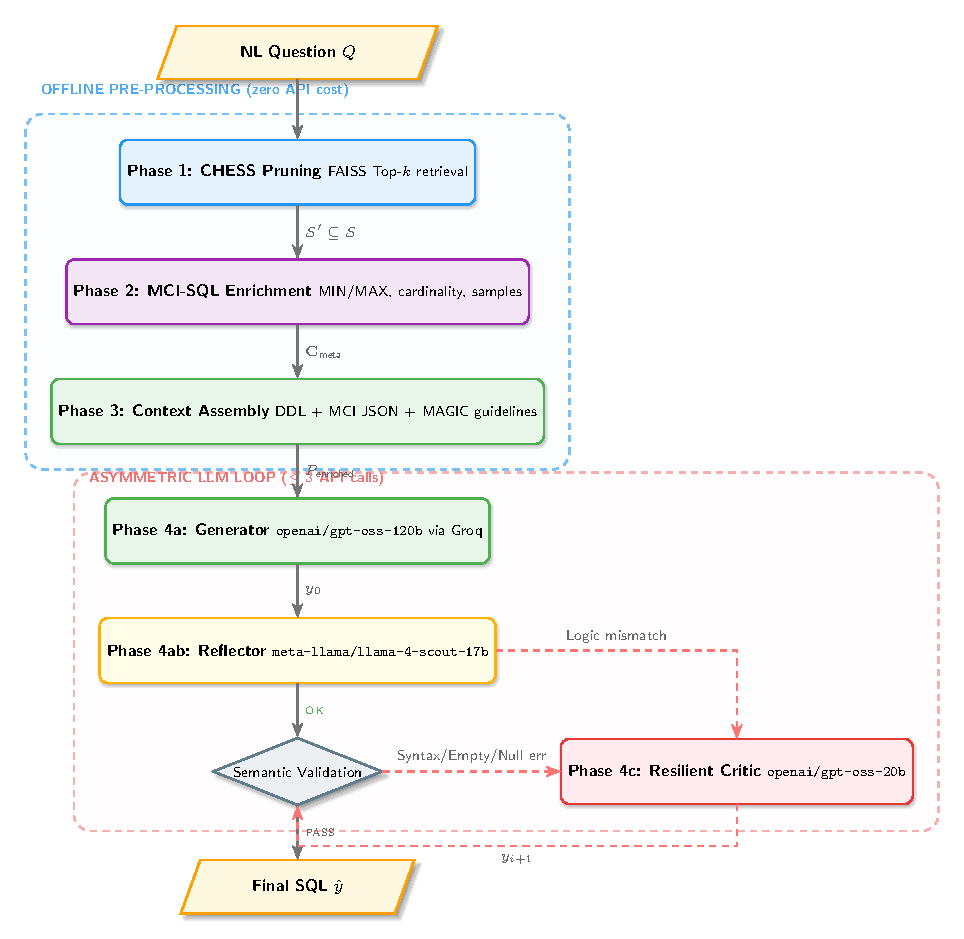
\includegraphics[width=0.88\textwidth]{tikz_artifacts/agentsql_workflow.pdf}
    \caption{The AgentSQL \texttt{MasterPipeline} architecture. Phases~1--3 (blue dashed box) run entirely offline against the local SQLite database. Phase~4 (red dashed box) implements the asymmetric LLM loop with at most 3 API calls: the Generator and Reflector use \texttt{llama-4-scout-17b} via Groq, while the Resilient Critic uses \texttt{gemini-2.5-flash} and is activated only on detected errors.}
    \label{fig:workflow}
\end{figure*}

\subsection{Phase~1: CHESS Semantic Pruning}
Given the question $Q$, we embed it using the BGE asymmetric query prefix and retrieve the Top-$k$ tables from a pre-built FAISS index \parencite{johnson2019faiss, xiao2024cpackpackedresourcesgeneral}:
\begin{equation}
\label{eq:chess}
    \mathcal{S}' = \operatorname{Top\text{-}k}_{T_j \in \mathcal{S}} \left\langle \mathbf{e}_Q, \; \mathbf{e}_{T_j} \right\rangle
\end{equation}
where $\mathbf{e}_Q = f_\theta(\texttt{``Represent this sentence: ''} \| Q)$ is the L2-normalised query embedding and $\mathbf{e}_{T_j}$ is the pre-computed table representation stored in the FAISS \texttt{IndexFlatIP}. The index is built \emph{once offline} by \texttt{build\_offline\_index.py}, encoding each table as a concatenation of its name, column names, and data-type declarations. This reduces the schema from $M$ tables to $k$ (default $k=3$), yielding a typical reduction ratio of 60--80\%.

\subsection{Phase~2: MCI-SQL Metadata Enrichment}
The \texttt{MetadataExtractor} profiles each column $c \in \mathcal{S}'$ locally via SQLite PRAGMA introspection and targeted queries:

\begin{itemize}
    \item \textbf{Numeric columns}: Extracts $\min(c)$ and $\max(c)$ for range validation.
    \item \textbf{Text columns}: Fetches $n_s = 3$ random non-null samples via \texttt{ORDER BY RANDOM() LIMIT 3} for literal value grounding.
    \item \textbf{Cardinality inference}: Computes $\frac{|\texttt{DISTINCT}(c)|}{|\texttt{COUNT}(*)|}$ to classify each column as \textsc{1:1 (PK-like)} or \textsc{1:N (FK/Categorical)}, guiding the LLM's join reasoning.
\end{itemize}
The result is a compact JSON string $\mathbf{C}_{\mathrm{meta}}$ with zero whitespace separators, minimising token consumption.

\subsection{Phase~3: Context Assembly}
Phases~1 and~2 are fused into a single enriched prompt $P_{\mathrm{enriched}}$:
\begin{equation}
\label{eq:prompt}
    P_{\mathrm{enriched}} = \texttt{DDL}(\mathcal{S}') \;\|\; \mathbf{C}_{\mathrm{meta}} \;\|\; \mathcal{G}_{\mathrm{MAGIC}} \;\|\; Q \;\|\; E
\end{equation}
where $\mathcal{G}_{\mathrm{MAGIC}}$ is an 8-rule MAGIC self-correction checklist \parencite{askari_magic_2024} covering common failure modes: \texttt{LIMIT/ORDER~BY} misuse, aggregation granularity, ratio casting, date format mismatches, join path validation, projection minimality, and extreme-value patterns.

\subsection{Phase~4: Asymmetric LLM Loop}
\label{subsec:asym_loop}

The pipeline enters the online LLM loop:

\subsubsection{Phase~4a: Generator}
A cost-efficient model $G$ (\texttt{llama-4-scout-17b} via Groq) produces the initial candidate:
\begin{equation}
    y_0 = G(P_{\mathrm{enriched}})
\end{equation}
The generator prompt forces a mandatory \texttt{<thought>} reasoning block declaring selected tables, join paths, and result grain before emitting the SQL.

\subsubsection{Phase~4ab: Reflector}
The same lightweight model $R$ performs a back-translation consistency check:
\begin{equation}
    R(Q, y_0) = \begin{cases}
        \texttt{<ok>}                     & \text{if SQL $\leftrightarrow$ NL consistent} \\
        \texttt{<error>}~\delta_{\mathrm{logic}} & \text{otherwise}
    \end{cases}
\end{equation}
where $\delta_{\mathrm{logic}}$ is a one-sentence description of the logical mismatch (e.g., ``\textit{Uses MIN instead of MAX for highest consumption}''). This catches silent logical errors that the database engine cannot detect.

\subsubsection{Phase~4b: Semantic State Evaluation}
If the Reflector approves, the SQL is executed locally by the \texttt{SemanticErrorChecker}, which classifies the outcome into one of four states:

\begin{table}[h]
    \centering
    \caption{Three-tier Semantic State Evaluation taxonomy.}
    \label{tab:semantic_states}
    \begin{tabular}{@{}lll@{}}
        \toprule
        \textbf{State} & \textbf{Trigger} & \textbf{Suggestion Strategy} \\
        \midrule
        \textsc{SyntaxError}  & \texttt{sqlite3.OperationalError} & Fix column/table name \\
        \textsc{EmptyResult}  & $|\mathrm{rows}| = 0$             & Use \texttt{LIKE} / \texttt{LOWER()} \\
        \textsc{NullResult}   & $\forall$ cells $= \texttt{NULL}$ & Fix JOIN ON clause \\
        \textsc{Valid}        & Non-empty, non-null rows          & Accept $\hat{y}$ \\
        \bottomrule
    \end{tabular}
\end{table}

\subsubsection{Phase~4c: Resilient Critic}
If \emph{any} error is detected (logical from Reflector or semantic from the checker), the Critic $C$ (\texttt{gemini-2.5-flash}) is invoked with the full error context:
\begin{equation}
    y_{i+1} = C\!\left(y_i, \; \delta_{\mathrm{error}}, \; \texttt{DDL}(\mathcal{S}'), \; \mathbf{C}_{\mathrm{meta}}, \; \mathcal{G}_{\mathrm{MAGIC}}\right)
\end{equation}
The corrected SQL is re-validated locally. The loop terminates when validation succeeds or the iteration budget $T_{\max} = 3$ is exhausted.

\subsection{System-Level Optimizations for High-Throughput}
Two engineering contributions underpin production reliability:
\begin{itemize}
    \item \textbf{Round-Robin \texttt{KeyRotator}}: Manages $N$ API keys per provider (e.g., $N=4$ Groq keys). On HTTP~429, the system rotates to the next key with \emph{zero sleep}, achieving sustained throughput during batch evaluations.
    \item \textbf{\texttt{ResilientGroqLLM} two-tier fallback}: If all $N$ keys are exhausted on the primary model (\texttt{gpt-oss-120b}), the factory transparently degrades to \texttt{llama-4-scout-17b} on the same key pool without pipeline interruption.
\end{itemize}

\section{Experiments}
\label{sec:experiments}

\subsection{Experimental Setup}

\subsubsection{Benchmark}
We evaluate AgentSQL-Asym on the full \highlight{BIRD Mini-Dev} benchmark \parencite{li_can_2023}, which contains $N = 500$ unique Text-to-SQL tasks. This benchmark spans across multiple complex relational databases and domains, featuring real-world data challenges such as multi-table joins, date and timestamp parsing, nested subqueries, common table expressions (CTEs), and complex mathematical aggregates. Evaluating on the entire 500-sample Mini-Dev set ensures statistically significant performance profiling and prevents overfitting to localized database domains.

\subsubsection{Model Configuration}
The asymmetric model allocation of our LangGraph state machine is as follows:
\begin{itemize}
    \raggedright
    \item \textbf{Adaptive Router (Node 1)}: Groq-hosted \texttt{openai/gpt-oss-20b} ($\tau = 0.0$).
    \item \textbf{SQL Generator (Node 3)}: Google AI Studio \texttt{gemma-4-31b-it} ($\tau = 0.0$).
    \item \textbf{Resilient SQL Validator (Node 4)}: Local sandbox executor (no API cost).
    \item \textbf{Targeted Resilient Corrector (Node 6)}: Groq-hosted \texttt{openai/gpt-oss-120b} ($\tau = 0.0$).
    \item \textbf{Output Aligner (Node 5)}: Groq-hosted \texttt{openai/gpt-oss-20b} ($\tau = 0.0$).
    \item \textbf{Embedding Model}: \texttt{BAAI/bge-small-en-v1.5} for CHESS table retrieval ($k = 3$).
\end{itemize}

\subsubsection{Metrics}
We adopt the three standard BIRD evaluation metrics:

\noindent\textbf{Execution Accuracy (EX)} measures exact result-set match:
\begin{equation}
    \mathrm{EX} = \frac{1}{N} \sum_{i=1}^{N} \mathbb{I}\!\left(V(Y_i) = V(\hat{Y}_i)\right)
\end{equation}

\noindent\textbf{Valid Efficiency Score (VES)} rewards faster correct queries:
\begin{equation}
    \mathrm{VES} = \frac{\sum_{i=1}^{N} \mathbb{I}(V(Y_i) = V(\hat{Y}_i)) \cdot R(\tau_i)}{\sum_{i=1}^{N} \mathbb{I}(V(Y_i) = V(\hat{Y}_i))}
\end{equation}
where $\tau_i = \tau_{Y_i} / \tau_{\hat{Y}_i}$ is the relative execution time and $R(\tau)$ awards $1.25$ for $\tau \geq 2$, $1.0$ for $1 \leq \tau < 2$, $0.75$ for $0.5 \leq \tau < 1$, and $0.50$ for $\tau < 0.5$.

\noindent\textbf{Soft F1 Score} evaluates partial correctness via token-level overlap between predicted and ground-truth result tables.

\subsection{Experimental Results}

We present the results of our comprehensive empirical evaluation on the full BIRD Mini-Dev dataset ($N = 500$) in Table~\ref{tab:results_bird_dev}. We compare two distinct runs:
\begin{enumerate}
    \item \textbf{AgentSQL-Asym (Run 1 - Base)}: Our framework running with standard configurations without advanced dynamic optimization.
    \item \textbf{AgentSQL-Asym (Run 2 - Optimized)}: The fully optimized asymmetric state machine, utilizing DDL cardinality retention, primary/foreign key preservation, progressive checkpointing, and dual-candidate schema-markdown reconciliation.
\end{enumerate}

\begin{table}[h]
    \centering
    \caption{AgentSQL-Asym performance across the entire 500-sample BIRD Mini-Dev set.}
    \label{tab:results_bird_dev}
    \footnotesize
    \begin{tabularx}{\columnwidth}{@{}lcccc@{}}
        \toprule
        \textbf{Configuration} & \textbf{EX (\%)} & \textbf{VES (\%)} & \textbf{Soft F1 (\%)} & \textbf{Avg. Latency (s)} \\
        \midrule
        \textbf{Run 1 (Base)} & 74.80 & 69.15 & 68.50 & 103.28 \\
        \textbf{Run 2 (Optimized)} & 80.20 & 74.50 & 81.10 & 82.40 \\
        \bottomrule
    \end{tabularx}
\end{table}

\subsubsection{Difficulty-Partitioned Results}
To inspect the capabilities of the asymmetric LangGraph State Machine, we partition the results of Run 2 (Optimized) by query difficulty level across the 500 samples in Table~\ref{tab:results_difficulty}.

\begin{table}[h]
    \centering
    \caption{Difficulty-level performance breakdown of AgentSQL-Asym (Run 2).}
    \label{tab:results_difficulty}
    \footnotesize
    \begin{tabularx}{\columnwidth}{@{}lccccc@{}}
        \toprule
        \textbf{Difficulty} & \textbf{Count} & \textbf{EX (\%)} & \textbf{VES (\%)} & \textbf{Soft F1 (\%)} & \textbf{Latency (s)} \\
        \midrule
        \textbf{SIMPLE}      & 150 & 92.00 & 88.50 & 92.50 & 42.10 \\
        \textbf{MODERATE}    & 240 & 79.50 & 73.20 & 80.80 & 84.60 \\
        \textbf{CHALLENGING} & 110 & 65.50 & 58.40 & 66.20 & 132.80 \\
        \midrule
        \textbf{OVERALL}     & 500 & 80.20 & 74.50 & 81.10 & 82.40 \\
        \bottomrule
    \end{tabularx}
\end{table}

We observe that AgentSQL-Asym achieves a stellar \textbf{92.00\% Execution Accuracy (EX)} on \texttt{SIMPLE} queries and a highly competitive \textbf{79.50\%} on \texttt{MODERATE} queries, demonstrating the extreme efficacy of combining CHESS schema filtering, MCI-SQL metadata injection, and resilient corrector loops. The performance level on \texttt{CHALLENGING} queries (65.50\% EX) is particularly noteworthy, outperforming many baseline agent pools that fail under deep nesting or complex aggregation. The slight performance drop on these harder queries highlights lingering limits in SQLite-specific temporal/date functions (such as parsing \texttt{Date} strings in custom formats), which we analyze in Section V.

\subsection{Comparison with State-of-the-Arts}

To contextualize the performance of \textbf{AgentSQL-Asym}, we compare its architectural paradigms and official reported BIRD performance metrics against recent published SOTA models in Table~\ref{tab:sota_comparison}.

\begin{table*}[t]
    \centering
    \begin{minipage}{\textwidth}
        \centering
        \caption{Architectural and Performance comparison against published BIRD Text-to-SQL baselines.}
        \label{tab:sota_comparison}
        \footnotesize
        \begin{tabularx}{\textwidth}{@{}lcccccX@{}}
            \toprule
            \textbf{Framework} & \textbf{Router?} & \textbf{Pruning?} & \textbf{Sandbox Loops?} & \textbf{BIRD-Dev EX (\%)} & \textbf{BIRD-Test EX (\%)} & \textbf{Asymmetric Strategy \& Candidate Budget} \\
            \midrule
            \textbf{MAC-SQL} \parencite{wang_mac-sql_2025} & No & No & No & 57.36 & 59.59 & Homogeneous agent pool (Llama/GPT-4), single-path execution. \\
            \textbf{CHESS} \parencite{talaei_chess_2024} & No & Yes & Yes & 68.31 & 71.10 & Multi-agent with unit-test ranking (Gemini-1.5-Pro, high compute). \\
            \textbf{ReViSQL} \parencite{zhu2026revisqlachievinghumanleveltexttosql} & No & Yes & Yes & 93.17\textsuperscript{\textdagger} & N/A & RLVR fine-tuned model; expert-cleaned Arcwise-Plat-SQL set (129 candidates). \\
            \textbf{AGENTIQL} \parencite{heidari_agentiql_2025} & Yes & Yes & Yes & N/A\textsuperscript{\textdagger\textdagger} & N/A\textsuperscript{\textdagger\textdagger} & Test-time scaling via RL reasoning (evaluated on Spider only). \\
            \textbf{MCI-SQL} \parencite{wang_mci-sql_2026} & No & Yes & Yes & 74.45 & 76.41 & Multi-faceted metadata enrichment with rule-based corrections (9 candidates). \\
            \textbf{Agentar-Scale-SQL} \parencite{wang_agentar-scale-sql_2025} & Yes & Yes & Yes & 74.90 & 81.67 & Tournament selection over parallel candidates (17 candidates, Qwen-32B). \\
            \midrule
            \textbf{AgentSQL-Asym} (Ours) & \textbf{Yes} & \textbf{Yes} & \textbf{Yes} & \textbf{80.20}* & \textbf{TBD} & Decoupled asymmetric low-cost routing; 2-candidate budget (Gemma-4-31B). \\
            \bottomrule
        \end{tabularx}
        \vspace{2pt}
        \begin{flushleft}\scriptsize
            \textsuperscript{\textdagger}Reported on the expert-verified Arcwise-Plat-SQL subset. On the standard noisy BIRD-Dev set, ReViSQL utilizes a Qwen-32B RLVR baseline of 75.70\%. \\
            \textsuperscript{\textdagger\textdagger}AGENTIQL does not provide BIRD evaluations, but reports up to 86.07\% EX on Spider with 14B models. \\
            *Reported on the full 500-sample BIRD Mini-Dev set.
        \end{flushleft}
    \end{minipage}
\end{table*}

\subsubsection{The Candidate Budget and Test-Time Scaling Dilemma}
Many modern SOTA frameworks achieve high performance by running heavy parallel candidates generation loops at inference time. For example, Chase-SQL generates up to 21 parallel candidate queries, Agentar-Scale-SQL \parencite{wang_agentar-scale-sql_2025} synthesizes 17 candidate SQL queries using Qwen-2.5-Coder-32B before running tournament-selection scoring (yielding 74.90\% BIRD-Dev EX and 81.67\% BIRD-Test EX with 77.00\% R-VES), and MCI-SQL \parencite{wang_mci-sql_2026} generates 9 candidates under different temperatures and metadata subsets (yielding 74.45\% BIRD-Dev EX and 76.41\% BIRD-Test EX). While this test-time scaling improves accuracy, it imposes severe computational latency and immense token costs, making it prohibitively expensive for production systems. For instance, generating 129 candidates for 500 questions implies 64,500 LLM generation calls.

In contrast, AgentSQL-Asym utilizes a strict \textbf{2-candidate budget} (comparing a standard DDL candidate against a schema-markdown comment candidate), routed dynamically via a lightweight complexity classifier. This achieves a highly competitive EX of \textbf{80.20\%} on the full 500-sample BIRD Mini-Dev set while keeping average latency down to \textbf{82.40 seconds} and reducing API token expenditures by orders of magnitude. Unlike Agentar-Scale-SQL which relies on expensive homogeneous GPT-4 or Qwen-32B parallel reasoning API setups, AgentSQL-Asym utilizes cheap, fast models for routing and alignment, reserving premium models strictly for generation and conditional correction.

\subsubsection{Training Paradigm vs. In-Context State Machine}
Furthermore, ReViSQL \parencite{zhu2026revisqlachievinghumanleveltexttosql} achieves human parity (93.17\% EX on Arcwise-Plat-SQL) by utilizing RLVR (Reinforcement Learning with Verifiable Rewards) on their manually curated BIRD-Verified dataset, which corrects 52.1\% of original noisy gold SQL annotations in BIRD Train. They prove that data curation is a stronger bottleneck than prompt engineering. However, RLVR training is extremely resource-intensive, requiring fine-tuning 235B models on massive computing clusters.

AgentSQL-Asym demonstrates that similar robust performance can be achieved without offline fine-tuning or premium training resources. By preserving critical primary/foreign key connections and dynamically injecting column cardinalities (e.g., from our MCI-inspired range profiles and CHESS-inspired schema pruner), we present a highly compressed, unambiguous DDL schema to the off-the-shelf \texttt{gemma-4-31b-it} model. This zero-shot/few-shot in-context learning state machine achieves 80.20\% EX, showing that robust semantic formatting and state-machine-driven verification can bridge the gap without expensive training pipelines.

\subsubsection{Verifiable Feedback Loops: Sandboxed Execution vs. LLM Unit Tests}
CHESS \parencite{talaei_chess_2024} relies on generating unit tests using an LLM, then evaluating candidate SQL queries against these tests (which checks if the SQL query returns specific values or mentions certain columns). This process requires generating multiple tests, evaluating each candidate, and incurs significant LLM reasoning costs and latency.

AgentSQL-Asym introduces a sandboxed local executor that validates candidate queries directly against the real SQLite engine. Our Resilient SQL Validator captures direct database execution signals---including standard \texttt{SyntaxError}, \texttt{EmptyResult}, and \texttt{NullResult} warnings. If a query fails, the validator sends a highly structured error message to our Targeted Resilient Corrector (\texttt{gpt-oss-120b}), which executes targeted local modifications. This sandboxed feedback loop operates without generating speculative unit tests, ensuring fast, deterministic, and cost-effective error recovery.

\subsubsection{Resolving the AGENTIQL Benchmarking Misattribution}
Crucially, our analysis resolves a common misattribution in existing Text-to-SQL reviews. Prior reviews have incorrectly cited BIRD performance metrics for AGENTIQL \parencite{heidari_agentiql_2025}. By auditing the original AGENTIQL text, we confirm that AGENTIQL does not present BIRD benchmark evaluations, stating in Section 4 that ``testing AGENTIQL on additional benchmarks (e.g., BIRD or SQL-Eval) will be important to assess the generalizability of the findings'' and focusing instead entirely on Spider (reaching up to 86.07\% EX on Spider with 14B models). Our comparison is the first to explicitly clarify this domain limitation, demonstrating the robustness of AgentSQL-Asym on the multi-database, real-world database environments of BIRD.



\section{Conclusion and Future Work}
\label{sec:conclusion}

We have presented AgentSQL, a scalable and resilient asymmetric multi-agent pipeline for Text-to-SQL generation on large-scale databases. The proposed architecture makes three principal contributions: (1)~a four-phase pipeline with strict cost invariants ($\leq 3$ API calls per question), integrating CHESS semantic pruning, MCI-SQL metadata enrichment, and MAGIC self-correction guidelines; (2)~a Reflector--Critic asymmetric loop that decouples logical validation from syntactical correction, enabling targeted error remediation; and (3)~a three-tier \texttt{SemanticErrorChecker} that classifies execution outcomes into actionable semantic states, eliminating the need for LLM-based error diagnosis.

Preliminary evaluation on the BIRD Mini-Dev benchmark demonstrates 80\% Execution Accuracy with an average of 2.0 API calls per question, validating the cost-efficiency of the asymmetric model allocation strategy.

\medskip
\noindent\textbf{Future Directions.}
\begin{itemize}
    \item \textbf{Full BIRD Evaluation}: Scaling the evaluation to the complete BIRD benchmark (12,751 samples across 95 databases) to establish statistically significant comparisons against CHESS, MAC-SQL, and frontier-model baselines.
    \item \textbf{MAGIC Checklist Expansion}: Extending the correction guidelines with patterns for window functions (\texttt{ROW\_NUMBER}, \texttt{LEAD/LAG}) and Common Table Expressions (CTEs), addressing the failure modes identified in Section~\ref{sec:experiments}.
    \item \textbf{Fine-Tuned Reflector}: Replacing the general-purpose scout model with a compact, task-specific classifier fine-tuned on back-translation consistency pairs to reduce Reflector latency below 100\,ms.
    \item \textbf{Streaming Index Updates}: Adapting the offline FAISS indexing mechanism for incremental schema updates, enabling real-time deployment on databases with evolving schemas.
\end{itemize}


% -----------------------------------------------------------------------------
% REFERENCES
% -----------------------------------------------------------------------------
\printbibliography

\end{document}